\subsection{Density Estimation}
\label{sec:density}

We use a histogram to estimate the merger rate as a function of $\mathcal{M}_c$, using Knuth's rule to determine the bin size (See Figure \ref{fig:chirp}). Since we are interested in the intrinsic rate, not just that of detected events, we weigh each point by the inverse of the spacetime volume in which we are sensitive to it, $w = 1 / VT$. Binaries with a higher chirp mass are easier to detect, so we do not want to count them as heavily. For a given chirp mass, we are sensitive out to a distance
%
\begin{equation}
  D(\mathcal{M}_c) =
  \SI{200}{\mega\parsec} \qty( \mathcal{M}_c / \SI{1.2}{\Msun} )^{5/6}
\end{equation}
%
which corresponds to a volume
%
\begin{equation}
  V(\mathcal{M}_c) = \frac{4}{3} \pi D^3(\mathcal{M}_c).
\end{equation}
%
Multiplying this by the time spent observing, $T = \SI{0.6}{yr}$, gives us the spacetime volume $V(\mathcal{M}_c) T$.

To obtain uncertainties in our histogram, we take the square root of the sum-of-squares of the weights within that bin, i.e.
%
\begin{equation}
  \sigma_k = \sqrt{\sum_i w_i^2},
\end{equation}
%
which was taken from \textcite{weighted-hist}. This reduces to $\sqrt{N}$ in the case of an unweighted histogram, as $w_i = 1$, so $\sum_i w_i^2 = N$.

We also over-plot a pure power law. To do this, we employ Bayesian linear regression, fitting a straight line to $\log r$ versus $\log \mathcal{M}_c$, and transforming back to linear space. This is also shown in Figure \ref{fig:chirp}.

\begin{figure*}[ht]
  \centering
  \begin{subfigure}[c]{\textwidth}
    \centering
    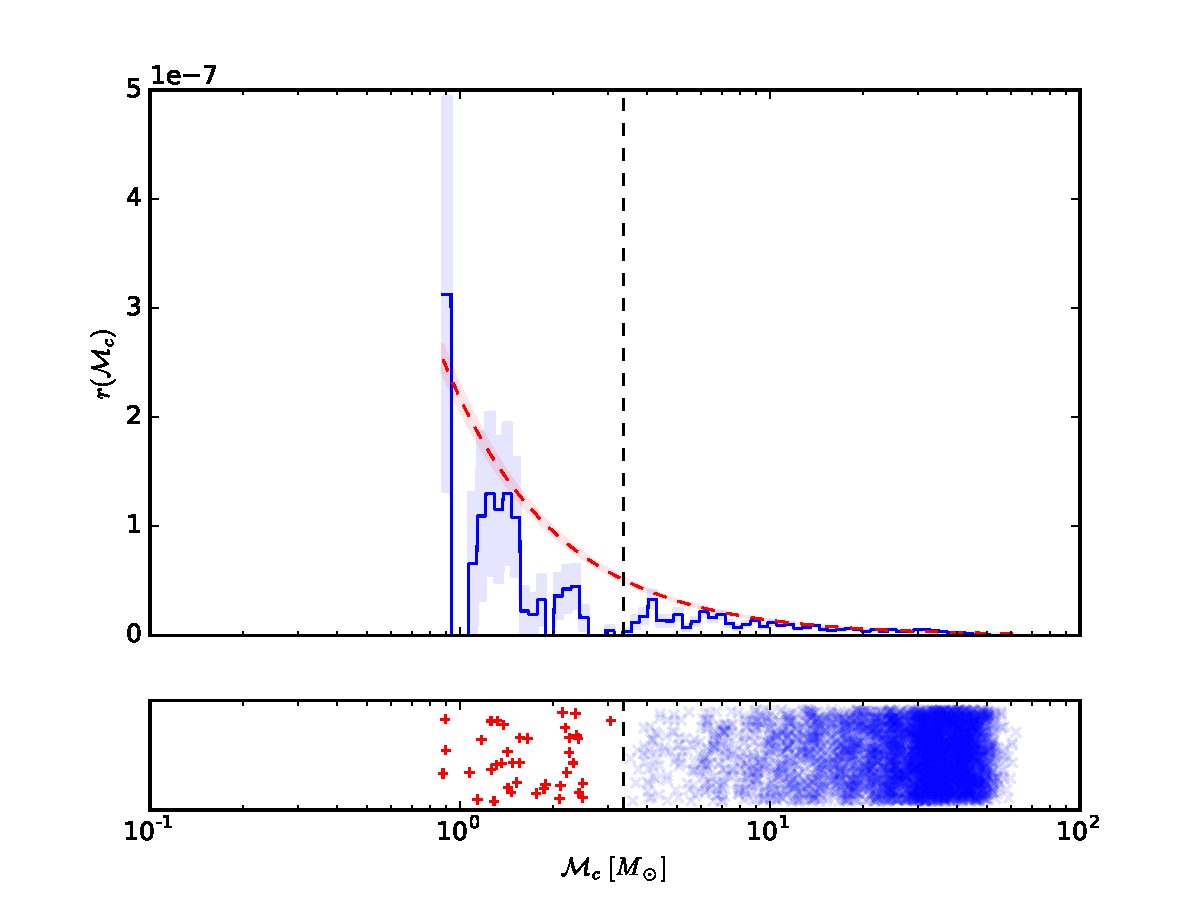
\includegraphics[height=0.4\textheight]{img/chirp-mass-distribution}
    \caption{}
    \label{fig:chirp-linear}
  \end{subfigure}

  \begin{subfigure}[c]{\textwidth}
    \centering
    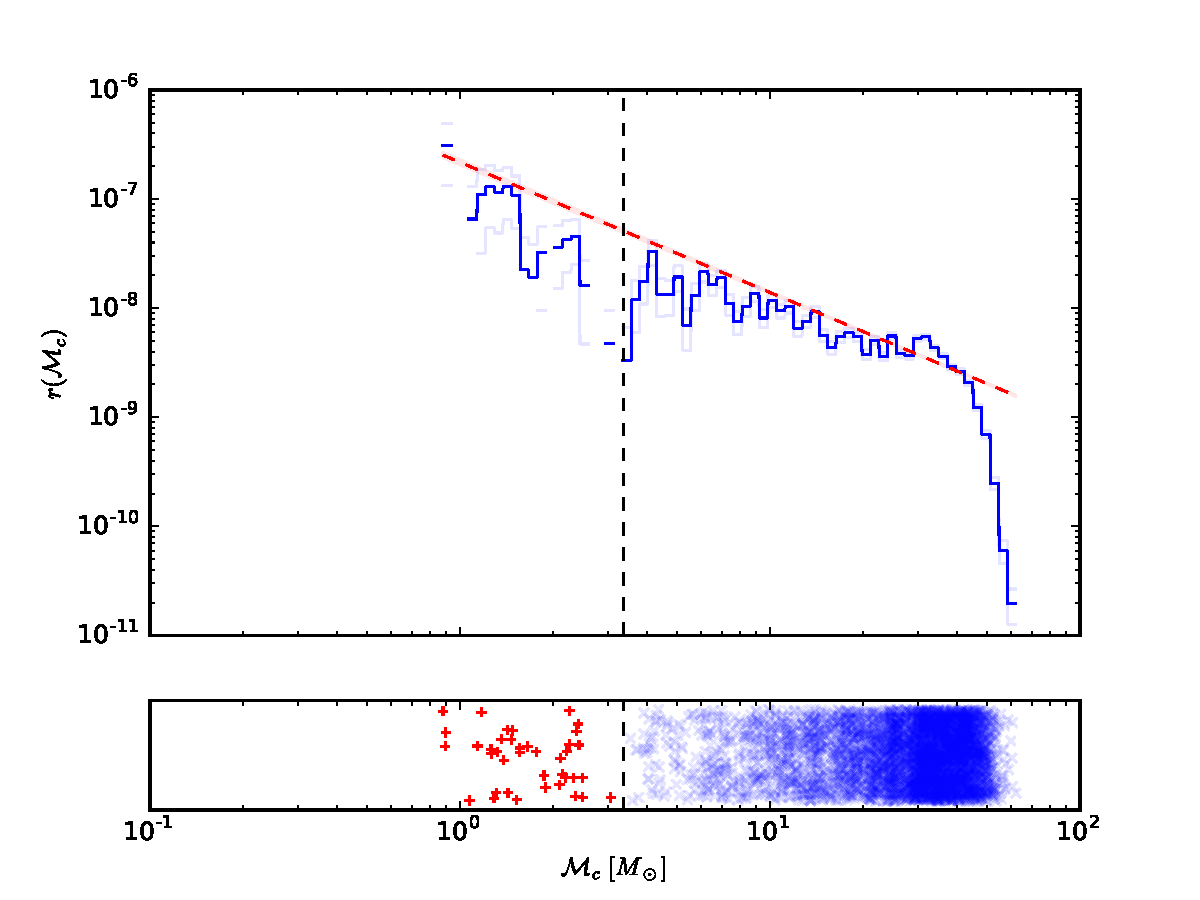
\includegraphics[height=0.4\textheight]{img/chirp-mass-log-distribution}
    \caption{}
    \label{fig:chirp-log}
  \end{subfigure}

  \caption{Estimated rate of compact binary mergers, based on 5000 synthetic observations. Rate is shown in (\subref{fig:chirp-linear}) linear and (\subref{fig:chirp-log}) log scale. Blue line is weighted histogram fit. Red curve is power law fit. Shaded regions are 1-$\sigma$ error bars. Vertical dashed line is boundary between events with counterparts and without.}
  \label{fig:chirp}
\end{figure*}